\documentclass[10.5pt]{article}
\usepackage{amsmath,amssymb,amsthm}
\usepackage{listings}
\usepackage{graphicx}
\usepackage[shortlabels]{enumitem}
\usepackage{tikz}
\usepackage[margin=1in]{geometry}
\usepackage{fancyhdr}
\usepackage{epsfig} %% for loading postscript figures
\usepackage{amsmath}
\usepackage{float}
\usepackage{amssymb}
\usepackage{caption}
\usepackage{subfigure}
\usepackage{graphics}
\usepackage{titlesec}
\usepackage{mathrsfs}
\usepackage{amsfonts}
\usepackage{indentfirst}
\usepackage{color}
\usepackage{soul}

\renewcommand{\baselinestretch}{1.2}%Adjust Line Spacing
%\geometry{left=2.0cm,right=2.0cm,top=2.0cm,bottom=2.0cm}% Adjust Margins of the File
\usepackage{tikz-qtree}
\usetikzlibrary{graphs}
\usetikzlibrary{arrows.meta}
\tikzset{every tree node/.style={minimum width=2em,draw,circle},
	blank/.style={draw=none},
	edge from parent/.style=
	{draw,edge from parent path={(\tikzparentnode) -- (\tikzchildnode)}},
	level distance=1.2cm}
\setlength{\parindent}{0pt}
%\setlength{\parskip}{5pt plus 1pt}
\setlength{\headheight}{13.6pt}
\newcommand\question[2]{\vspace{.25in}\hrule\textbf{#1: #2}\vspace{.5em}\hrule\vspace{.10in}}
\renewcommand\part[1]{\vspace{.10in}\textbf{(#1)}}
\newcommand\algorithm{\vspace{.10in}\textbf{Algorithm: }}
\newcommand\correctness{\vspace{.10in}\textbf{Correctness: }}
\newcommand\runtime{\vspace{.10in}\textbf{Running time: }}
\pagestyle{fancyplain}
% Create horizontal rule command with an argument of height
\newcommand{\horrule}[1]{\rule{\linewidth}{#1}}



% Set the title here
\title{
	\normalfont \normalsize
	\textsc{ShanghaiTech University} \\ [25pt]
	\horrule{0.5pt} \\[0.4cm] % Thin top horizontal rule
	\huge CS101 Algorithms and Data Structures\\ % The assignment title
	\LARGE Fall 2021\\
	\LARGE Homework 8\\
	\horrule{2pt} \\[0.5cm] % Thick bottom horizontal rule
}
% wrong usage of \author, never mind
\author{}
\date{Due date: 23:59, November 28, 2021}

% set the header and footer
\pagestyle{fancy}
\lhead{CS101 Algorithms and Data Structures}
\chead{Homework 8}
\rhead{Due date: 23:59, November 28, 2021}
\cfoot{\thepage}
\renewcommand{\headrulewidth}{0.4pt}
\newtheorem{Q}{Question}
% special settings for the first page
\fancypagestyle{firstpage}
{
	\renewcommand{\headrulewidth}{0pt}
	\fancyhf{}
	\fancyfoot[C]{\thepage}
}

% Add the support for auto numbering
% use \problem{title} or \problem[number]{title} to add a new problem
% also \subproblem is supported, just use it like \subsection
\newcounter{ProblemCounter}
\newcounter{oldvalue}
\newcommand{\problem}[2][-1]{
	\setcounter{oldvalue}{\value{secnumdepth}}
	\setcounter{secnumdepth}{0}
	\ifnum#1>-1
	\setcounter{ProblemCounter}{0}
	\else
	\stepcounter{ProblemCounter}
	\fi
	\section{Problem \arabic{ProblemCounter}: #2}
	\setcounter{secnumdepth}{\value{oldvalue}}
}
\newcommand{\subproblem}[1]{
	\setcounter{oldvalue}{\value{section}}
	\setcounter{section}{\value{ProblemCounter}}
	\subsection{#1}
	\setcounter{section}{\value{oldvalue}}
}

% \setmonofont{Consolas}
\definecolor{blve}{rgb}{0.3372549 , 0.61176471, 0.83921569}
\definecolor{gr33n}{rgb}{0.29019608, 0.7372549 , 0.64705882}
\makeatletter
\lst@InstallKeywords k{class}{classstyle}\slshape{classstyle}{}ld
\makeatother
\lstset{language=C++,
	basicstyle=\ttfamily,
	keywordstyle=\color{blve}\ttfamily,
	stringstyle=\color{red}\ttfamily,
	commentstyle=\color{magenta}\ttfamily,
	morecomment=[l][\color{magenta}]{\#},
	classstyle = \bfseries\color{gr33n}, 
	tabsize=4
}
\lstset{basicstyle=\ttfamily}
\begin{document}

\maketitle
\thispagestyle{firstpage}
%\newpage
\vspace{3ex}

\begin{enumerate}
	\item Please write your solutions in English.

	\item Submit your solutions to gradescope.com.

	\item Set your FULL NAME to your Chinese name and your STUDENT ID correctly in Account Settings.

	\item If you want to submit a handwritten version, scan it clearly. Camscanner is recommended.

	\item When submitting, match your solutions to the according problem numbers correctly.

	\item No late submission will be accepted.

	\item Violations to any of the above may result in zero grade.
\end{enumerate}
\newpage

%%%%%%%%%%%%%%%%%%%%%%%%%%%%%
\question{1}{(4$\times$2') Choice}
The following \textit{} questions are choice questions, each question may have \textbf{one} or \textbf{multiple} correct answers. Select all the correct answer, you will get half points if you choose a strict subset(excluding empty set) of the right answer.\\
\textit{Note: You should write those answers \textbf{in the box} below.}

\begin{table}[htbp]
	\begin{tabular}{|p{2cm}|p{2cm}|p{2cm}|p{2cm}|}
		\hline
		Question 1 & Question 2 & Question 3 & Question 4 \\
		\hline
		B C        & A          & A B C D    & D          \\
		\hline
	\end{tabular}
\end{table}



\begin{Q}
	Which of the following statements are/is true?
	\begin{enumerate}[(A)]
		\item Prim's algorithm for computing a minimum spanning tree of a graph only works if the weights of the edges are non-negative.
		\item A minimum spanning tree for a connected graph has exactly $N-1$ edges, where $N$ is the number of vertices in the graph.
		\item A connected graph that has unique edge weights (there are \textbf{no} two edges with the same weight) has a unique minimum spanning tree.
		\item None of above is True
	\end{enumerate}
\end{Q}


\begin{Q}
	Which of the following statements are/is true?
	\begin{enumerate}[(A)]
		\item For Prim's algorithm, it is possible to calculate the minimum spanning tree of some graph in $\Theta(E)$ time without using priority queue and adjacent list. $E$ represents the number of edges in the graph.
		\item Kruskal's algorithm adds the least-weighted edge each time to the MST.
		\item The removal of any edge from an MST will not disconnect this MST.
		\item None of above is True.
	\end{enumerate}
\end{Q}


\begin{Q}
	You are given a connected undirected graph G with m distinct edges (distinct costs), in adjacency list representation. You are also given the edges of a minimum spanning tree T of G. This question asks how quickly you can recompute the MST if we change the cost of a single edge. Which of the following are/is true? (RECALL: The disjoint set data structure has run-time $O(\alpha (n))$, which is effectively a constant)
	\begin{enumerate}[(A)]
		\item Suppose e $\in$ T and we increase the cost of e. Then, the new MST can be recomputed in O(m) deterministic time.
		\item Suppose e $\notin$ T and we increase the cost of e. Then, the new MST can be recomputed in O(m) deterministic time.
		\item Suppose e $\in$ T and we decrease the cost of e. Then, the new MST can be recomputed in O(m) deterministic time.
		\item Suppose e $\notin$ T and we decrease the cost of e. Then, the new MST can be recomputed in O(m) deterministic time.
	\end{enumerate}
\end{Q}


\begin{Q}
	Consider the following algorithm that attempts to compute a minimum spanning tree of a connected undirected graph $G$ with distinct edge costs. First, sort the edges in decreasing cost order (i.e., the opposite of Kruskal's algorithm). Initialize $T$ to be all edges of $G$. Scan through the edges (in the sorted order), and remove the current edge from $T$ if and only if it lies on a cycle of $T$.\\
	Which of the following statements is true?
	\begin{enumerate}[(A)]
		\item The output of the algorithm will never have a cycle, but it might not be connected.
		\item The algorithm always outputs a spanning tree, but it might not be a minimum cost spanning tree.
		\item The output of the algorithm will always be connected, but it might have cycles.
		\item The algorithm always outputs a minimum spanning tree.
	\end{enumerate}
\end{Q}
\pagebreak

% ======================================

\question{2}{(8') Play with Prim and Kruskal}
Here we give the adjacent list of a DAG(Directed Acyclic Graph). The letters on the left of the arrows are the source vertices of the edges. The destination vertex $v$ and weights of the edge $w$ is given in the form of ${\boxed{v}\boxed{w}}$ on the right of the arrows.
\begin{align*}
	 & \boxed{A}\rightarrow\boxed{B}\boxed{3}\rightarrow\boxed{C}\boxed{5}\rightarrow\boxed{D}\boxed{2} \\
	 & \boxed{B}\rightarrow\boxed{C}\boxed{4}\rightarrow\boxed{D}\boxed{6}\rightarrow\boxed{E}\boxed{4} \\
	 & \boxed{C}\rightarrow\boxed{D}\boxed{2}                                                           \\
	 & \boxed{D}\rightarrow\boxed{E}\boxed{10}\rightarrow\boxed{F}\boxed{7}                             \\
	 & \boxed{E}\rightarrow\boxed{F}\boxed{3}                                                           \\
	 & \boxed{F}
\end{align*}

Suppose we start from vertex ``A''.\\
(1)(2') Draw the graph of the DAG with the adjacent list given above. Annotate the edges with their weight.\\
\begin{center}
	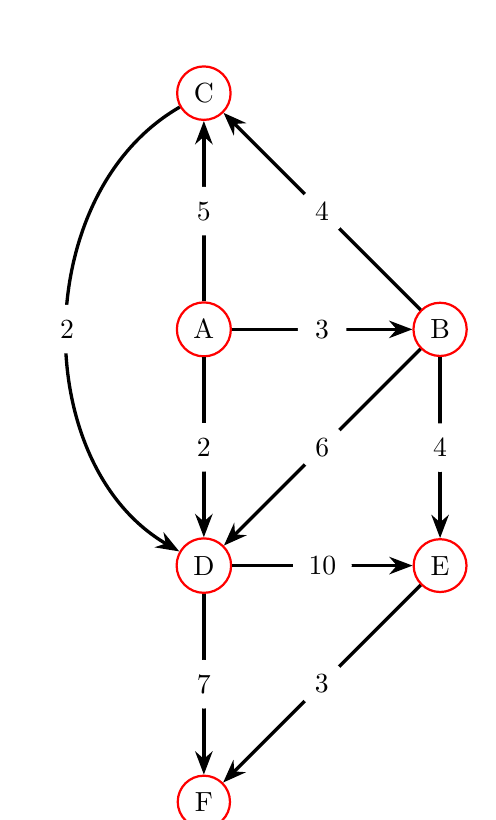
\begin{tikzpicture}
		\begin{scope}[every node/.style={circle,thick,draw=red}]
			\node (A) at (0,0) {A};
			\node (B) at (3,0) {B};
			\node (C) at (0,3) {C};
			\node (D) at (0,-3) {D};
			\node (E) at (3,-3) {E};
			\node (F) at (0,-6) {F};
		\end{scope}
		\begin{scope}[>={Stealth[black]},
			every node/.style={fill=white,circle},
			every edge/.style={draw,very thick}]
			\path [->] (A) edge node {$3$} (B);
			\path [->] (A) edge node {$5$} (C);
			\path [->] (A) edge node {$2$} (D);
			\path [->] (B) edge node {$4$} (C);
			\path [->] (B) edge node {$6$} (D);
			\path [->] (B) edge node {$4$} (E);
			\path [->] (C) edge[bend right=60] node{$2$} (D);
			\path [->] (D) edge node {$10$} (E);
			\path [->] (D) edge node {$7$} (F);
			\path [->] (E) edge node {$3$} (F);
		\end{scope}
	\end{tikzpicture}
\end{center}
(2)(2') View the DAG above as an undirected graph and draw its \textbf{maximum} spanning tree.\\
\begin{center}
	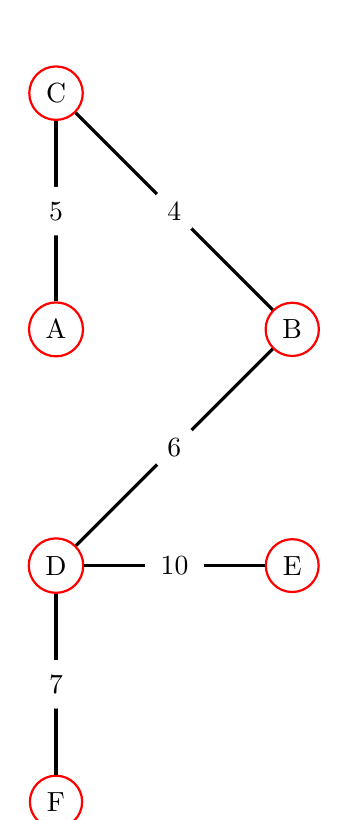
\begin{tikzpicture}
		\begin{scope}[every node/.style={circle,thick,draw=red}]
			\node (A) at (0,0) {A};
			\node (B) at (3,0) {B};
			\node (C) at (0,3) {C};
			\node (D) at (0,-3) {D};
			\node (E) at (3,-3) {E};
			\node (F) at (0,-6) {F};
		\end{scope}
		\begin{scope}[>={Stealth[black]},
			every node/.style={fill=white,circle},
			every edge/.style={draw,very thick}]
			\path [-] (A) edge node {$5$} (C);
			\path [-] (B) edge node {$4$} (C);
			\path [-] (B) edge node {$6$} (D);
			\path [-] (D) edge node {$10$} (E);
			\path [-] (D) edge node {$7$} (F);
		\end{scope}
	\end{tikzpicture}
\end{center}
(3)(2') Write down the sequence of edges added to the \textbf{maximum} spanning tree using Kruskal's algorithm.\\
$E(D, E), E(D, F), E(B, D), E(A, C), E(B, C)$

(4)(2') Write down the sequence of edges added to the \textbf{maximum} spanning tree using Prim's algorithm.\\
$E(A, C), E(B, C), E(B, D), E(D, F), E(D, F)$\\
\\\\\\

\pagebreak

% =========================
\question{3}{(12') Minimum Spanning Tree}

We are given the following graph $G$:

\begin{center}\includegraphics[scale=0.4]{3.jpg}
\end{center}

For each question below, please give your answer firstly and then explain it briefly.\\
\textbf{Note} that questions below are independent to each other. \\
(1)(2') For what range of values of $g$ are you \textbf{guaranteed} to include edge BE in the MST?\\
\\
$g< 8$\\
First, seperate the graph into two subset $S_1$ and $S_2$. Vertex $E$ is in $S_2$, and the rest are in $S_1$. Then edge BE and edge EF are the cut set of the graph. By cut property, if $g < 8$, BE must be included in the MST.\\
If $g \ge 8$, we use reverse kruskal algorithm introduced in Question 4, and sort the edges in descending weight order. Since $g$ is the biggest value, and remove BE will not disconnect the graph, edge BE will be removed at first and won't be in the MST.\\
Therefore, $g < 8$.\\
\\
(2)(2') For what range of values of $k$ are you \textbf{guaranteed} to include edge CD in the MST?.\\
$k<2$\\
\\
First, seperate the graph into two subset $S_1$ and $S_2$. Vertex $C$ is in $S_2$ and the rest are in $S_1$. Edge AC, CD and CG is the cut set of the graph. By cut property, if $k$ is the least among all the edge weights in the cut set (i.e. $k < 2$), CD will be included in the MST.\\
If $k \ge 2$, we use prim's algorithm to build the MST. Edge AD and AC will be add into the MST first, since their weights are smaller. Therefore edge CD won't be added into the MST because it will create a cycle.\\
Therefore, $l < 2$.\\
\\
(3)(2') For what range of values of $k$ are you \textbf{guaranteed to NOT} include edge CD in the MST?.\\
$k > 2$\\
We use prim's algorithm to build the MST, and sort the edges in ascending weight order. Edge AD and AC will be add into the MST first, because they have the least weight and adding them won't create a cycle on the graph. After that, edge CD won't be added in to the MST, since it will create an cycle.\\
If $k \le 2$, we use prim's algorithm to build the MST. AD and CD can be added into the MST first and this can't guarantee not to include CD in the MST.\\
Therefore, $k > 2$\\
\\
(4)(3') Suppose an adversary can set $g$ and $k$ arbitrarily. What is the maximum cost of a MST that the adversary can force?\\
18.\\
First, set $g$ and $k$ to infinitely large, and we can build the following MST:\\
\begin{center}
	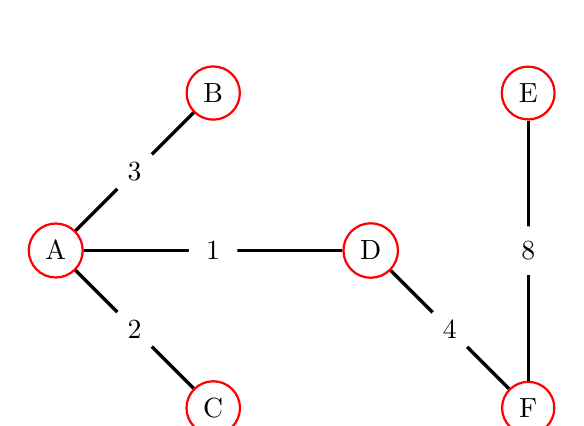
\begin{tikzpicture}
		\begin{scope}[every node/.style={circle,thick,draw=red}]
			\node (A) at (0,0) {A};
			\node (B) at (2,2) {B};
			\node (C) at (2,-2) {C};
			\node (D) at (4, 0) {D};
			\node (E) at (6,2) {E};
			\node (F) at (6,-2) {F};
		\end{scope}
		\begin{scope}[>={Stealth[black]},
			every node/.style={fill=white,circle},
			every edge/.style={draw,very thick}]
			\path [-] (A) edge node {$1$} (D);
			\path [-] (A) edge node {$2$} (C);
			\path [-] (A) edge node {$3$} (B);
			\path [-] (D) edge node {$4$} (F);
			\path [-] (E) edge node {$8$} (F);
		\end{scope}
	\end{tikzpicture}
\end{center}
And the total const is 18.\\
If we set $k \ge 2$, or set $g \ge 8$, CD and BE will not be select into the MST (or they won't change the total cost of the MST, if $k = 2$ or $g = 8$), so the total cost of the MST won't increase.
If we set $k < 2$, we will substitude CD for AC and the total cost will be
$$
	18 - 2 + k = 16 + k < 18
$$
If we set  $g < 8$, we will substitude BE for EF and the total cost will be
$$
	18 - 8 + k = 10 + k < 18
$$
Therefore, no matter which value we set for $k$ or $g$, we won't make the cost of MST bigger than $18$.\\
\\
(5)(3') Draw seven edges on the following graph with six vertices, and then mark six edges with cost=1 and one edge with cost=$x$ such that an adversary can choose $x$ such that the cost of the MST is arbitrarily large.
\begin{figure}[h]
	\centering
	\includegraphics[width=0.3\linewidth]{3-5}
\end{figure}

\begin{center}
	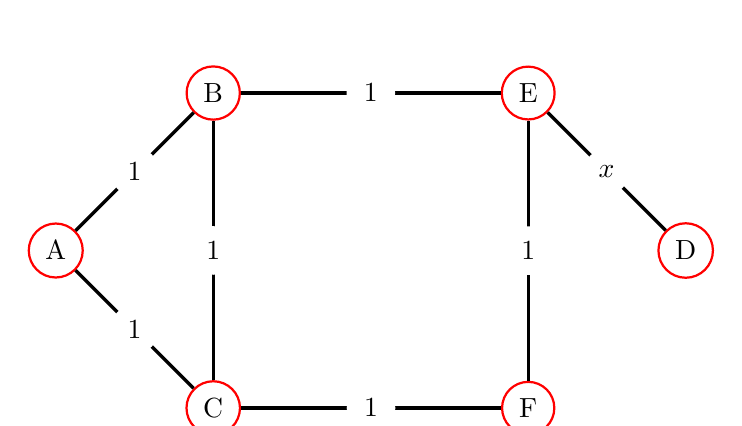
\begin{tikzpicture}
		\begin{scope}[every node/.style={circle,thick,draw=red}]
			\node (A) at (0,0) {A};
			\node (B) at (2,2) {B};
			\node (C) at (2,-2) {C};
			\node (D) at (8, 0) {D};
			\node (E) at (6,2) {E};
			\node (F) at (6,-2) {F};
		\end{scope}
		\begin{scope}[>={Stealth[black]},
			every node/.style={fill=white,circle},
			every edge/.style={draw,very thick}]
			\path [-] (A) edge node {$1$} (B);
			\path [-] (A) edge node {$1$} (C);
			\path [-] (B) edge node {$1$} (C);
			\path [-] (B) edge node {$1$} (E);
			\path [-] (C) edge node {$1$} (F);
			\path [-] (E) edge node {$1$} (F);
			\path [-] (E) edge node {$x$} (D);
		\end{scope}
	\end{tikzpicture}
\end{center}
Edge ED must be included in the MST, so $x$ can be set to an arbitrarily value while be guaranteed to be included in the MST. Therefore, the cost of MST can be arbitrarily large.\\

\pagebreak
\newpage
% =========================
\question{4}{(8') Building A Tower}
We build up a tower with a pile of stones. Each layer of the tower is exactly one
piece of stone. We index the layers from top to bottom, so layer 1 is the top
layer. The stone weight of the $i$-th layer is $s_i$. The tower will fall if there exists
a layer $i$ s.t. $\Sigma_{j=1} ^{i-1} s_j > s_i$. For example, if the tower is built with 5 stones and the stone weight from top to bottom is 2, 3, 5, 9, 100, then the tower would fall because $9 < 5 + 3 + 2 = 10$. \\
You are the designer of the tower and you have n stones. Each stone has different weight and the same height. Can you build the tower as high as possible?  Give an $O(nlogn)$ algorithm and prove that the algorithm produces the highest tower. Show the time complexity of your algorithm. Your answer should contain at least the following parts: \\
1. Main idea of your algorithm (which can also include pseudo-code here). (2')\\
2. Proof of the correctness of your algorithm. (4')\\
3. Time complexity analysis. (2')\\
\\
1.\\
Sort the stones in ascending weight order and build the tower from top to bottom. Iterate throught the stones, if the stone is heavier than the sum of seleted stone, then select the stone.\\
\begin{lstlisting}
function BuildATower(stones)
	Sort stones in ascending weight order;
	let total_weight = 0;
	let height = 0;
	for i = 1 to stones.length do
		if stones[i].weight >  total_weight
			total_weight += stones[i].weight;
			height++;
	return height;
\end{lstlisting}
2.\\
Sort the stones $S_n = \{s_1, s_2, ..., s_n\}$ in ascending weight order., where $s_1\le s_2\le \dots\le s_n$. Define greedy solution $T(S_n) = \{s_{t_1}, s_{t_2}, ..., s_{t_m}\}$, where $t_1 < t_2 < \dots < t_m, m\le n$.\\
\\We define function $W(T(S_k))$ is the total weight of the stones in the set $T(S_k)$.\\
First we need to prove, if two greedy $T(S_n)$ and another method $T^*(S_n)$ give the same height, then
$$
	W(T(S_n)) \le W(T^*(S_n))
$$
We find the first two inequal elements $s_i$ in $T(S_n)$ and $s^*_i$ in $T^*(S_n)$. Since greedy always choose the first element heavier than the sum of the weights of the previously selected stones,
$$
	W(\{s_i\}) \le W(\{s^*_i\})
$$
Then we can substitude $s_i$ for $s^*_i$ in $T^*(S_n)$ and the total weight of $T^*(S_n)$ decrease.\\
We select those elements iteratively until $T^*(S_n) = T^(S_n)$. We put all the $s_i$ into $X$, and all the $s^*_i$ into $X^*$. Then we have
$$
	W(T(S_n)) =W(T^*(S_n)) + W(X) - W(X^*) \le W(T^*(S_n))
$$
Next, we prove the greedy algorithm is optimal by induction.\\
\textbf{Base case:}\\
When $n = 1$, there's only one stone. Therefore $T(S_1)$ is optimal.\\
We suppose when $n = k$, $T(S_k)$ is optimal. We can prove when $n = k + 1$, $T(S_{k + 1})$ is also optimal by contradiction.\\
Suppose $T(S_{k+1})$ is not optimal, there exists an optimal solution $O(S_{k+1})$ includes $s_{k + 1}$ and $\left|O(S_{k + 1})\right| > \left|T(S_{k + 1})\right|$.
\\
If $s_{k + 1}\in T(S_{k + 1})$, then $\left|O(S_{k})\right| > \left|T(S_{k})\right|$, which means $O(S_k)$ is optimal when $n = k$. This is contradict to induction hypothesis.
\\
This can only happen when $s_{k + 1}\in O(S_{k+1})$ and $s_{k + 1}\notin T(S_{k + 1})$.\\
Let $O(S_{k}) = O(S_{k + 1})\setminus s_{k+1} \ne T(S_k)$ and $|O(S_{k})| = |T(S_k)|$.
There are two cases: $W(O(S_k))\ge W(T(S_k))$ and $W(O(S_k)) < W(T(S_k))$.\\
In the first case $O(S_{k + 1})$ can't include $s_{k + 1}$, because $T(S_{k + 1})$ can't include $s_{k + 1}$.
$$
	W(O(S_k))\ge W(T(S_k)) > W(\{s_{k + 1}\})
$$
This leads to a contradiction.\\
In the second case we have proved if two method give the same height, then the total weight of greedy algorithm must the least. This leads to a contradiction.\\
Therefore, when $n = k + 1$, greedy algorithm is still optimal.\\
By mathematical induction, we proved that greedy algorithm is the optimal algorithm.
\\
3.\\
First we have to sort the stones wich takes $O(n\log n)$.\\
We only need to go through the stones' weights once, so the time complexity of the loop is $O(n)$\\
Therefore, the time complexity of the algorithm is $O(n\log n)$

\pagebreak

% =========================
\question{5}{(9') To be A Grandparent}
Assume you are a grandparent and going to give your grandchildren some pieces of cake. However you cannot satisfy a child unless the size of cake piece he receives is no less than his expected size. Different children may have different expected sizes. Meanwhile, you can’t give each child more than one piece. For example, if three children’s expected sizes are {1, 3, 4} and the sizes of pieces of
cake are {1, 2}, then you could only satisfy the first child. Given the expected sizes of the children and the sizes of cake pieces that you have, how can you make the most children satisfied? Show that your algorithm is correct and analyze the time complexity. Same as Q4, your answer should contain at least the following parts: \\
1. Main idea of your algorithm (which can also include pseudo-code here). (3')\\
2. Proof of the correctness of your algorithm. (4')\\
3. Time complexity analysis. (2')\\
1.
\\
First, sort two list in descending order. Each time, remove the child who has bigger expected size than the biggest cake size. Then give the biggest cake to the child who has the biggest expected cake size.\\
\begin{lstlisting}
function ToBeAGrandParent(children, cakes):
	sort children in descending cake size order;
	sort cakes in descending cake size order;
	let pcake = 1, pchild = 1, ans = 0;
	while pcake <= cake.length and pchild <= children.length
		while pchild <= children.length and children[pchild].size > cakes[pcake].size
			pchild++;
		if pchild <= children.length
			ans++;
			pcake++;
			pchild++;
	return ans;
\end{lstlisting}
2.
\\
Sort the children and cakes in descending size order. Define the pair (h, c), h is the expected size of the children, and c is the cake size.
\\
Assume there is an optimal solution $O =\{(i_1, j_1), (i_2, j_2), \cdots, (i_m, j_m) \}$ and a solution from the greedy algorithm $T = \{(a_1, b_1), (a_2, b_2), \cdots, (a_k, b_k)\}$. $b_r \ge a_r$, $j_r \ge i_r$, $b_r \ge b_{r - 1}$, $j_r \ge g_{r-1}$ for all $r$. We will prove that $|O| = |A|$.\\
\textbf{Lemma 1:} $b_r \ge j_r$ for all $r$
\\
Since greedy always consit the cake with bigger size first, $b_1, b_2, \cdots, b_n$ is a consecutive subset of the give cakes, and $b_r \ge j_r$ for all $r$.\\
\\
\textbf{Lemma 2:} In the optimal solution $O$, $i_r$ can be rearranged in descending order and $i_{r-1} \ge i_r$.\\
If for any $k < r$, $i_k < i_r$. Because $j_k \ge j_r$ and $j_r\ge i_r$ so
$$
	i_r \le j_k
$$
Becuase $i_r \le j_r$, so
$$
	i_k < j_r
$$
Therefore, we can exchange $i_r$ and $i_k$, $O$ is still optimal.\\
\\
\textbf{Lemma 3:} In the solution given by greedy algorithm, $a_r$ is in descending order.\\
Greedy check the child with bigger expected cake size first, and $a_{r-1}$ is checked before $a_r$, so $a_{r - 1} > a_r$.
\\
\\
We will prove for all $r$, $a_r \ge i_r$ by mathematical induction.\\
\textbf{Base case:}\\
when $r = 1$, there's only one child get the cake. Since greedy always consider the cake with bigger size first, $b_1 \ge j_1$.
Greedy also choose the child with the possibly maximal expected cake size which is lesser than the cake size. $a_1 \ge i_1$.
\\
Assume $a_{r - 1}\ge i_{r - 1}$, prove $a_r \ge i_r$.\\
Suppose $a_r < i_r$. We know $b_{r-1}\ge a_{r-1}$, $a_{r-1} \ge i_{r-1}$. By \textbf{Lemma 2}, $i_{r-1}\ge i_r$. Therefore, we have
$$
	b_{r-1} \ge a_{r-1} \ge i_{r - 1} \ge i_r > a_r
$$
By defination, we know $j_r \ge i_r$. By \textbf{Lemma 1}, we know $b_r \ge j_r$.
Therefore,
$$
	b_r \ge j_r \ge i_r > a_r
$$
By \textbf{Lemma 3}, we know greedy didn't choose $i_r$ before $a_{r - 1}$ because $a$ should be in descending order. Therefore, greedy algorithm should choose $i_{r-1}$ rather than $a_r$. This is contradicted to the defination of the greedy algorithm.\\
Therefore, by mathematical induction, for all $r$, $a_r \ge i_r$.
\\
Next, we will prove that $|T| = |O|$.\\
$|T| = k, |O| = m$. Since $O$ is optimal, $m \ge k$. We will prove $m \le k$.\\
Suppose $m > k$, by the same reasoning as the induction earlier in this proof, we know
$$
	b_k \ge j_k \ge j_m \ge i_m
$$
$$
	a_k \ge j_k \ge i_m
$$
If the greedy algorithm continues, it will inculde $(i_m, j_m)$ since it doesn't conflict with the existing solution. This means $|T| \ne k$, which leads to a contradiction.\\
Therefore, $|T| = |O|$.
\\
3.
\\
Let $c$ be the length of the cakes list and $d$ be the length of the children list.
First, we have to sort the two list wich cost $O(n\log n)$($n = max(c, d)$).
Second, we only have to go through all the cake and and children, the loop cost $O(c + d)$.
Therefore, the time complexity is $O(n\log n)$


\end{document}